% v1.1, 2026-08-18: single-thesis revision for research-sample use.
% Governing claim: in base Qwen3.5-35B-A3B the redflag-minus-benign routing
% difference is led by one expert (173 at layer 25) atop a distributed
% consequence/duty set; suppressing that expert with a router bias collapses
% its routed mass dose-dependently while refusal persists and routing
% reallocates to the rest of the set. Implication: refusal-associated routing
% is distributed, so single-expert monitoring, ablation, or attack is not a
% sufficient audit or attack surface in this model; router-level safety
% telemetry should read expert sets. Changes from v1.0 (June 2026):
% two-column layout; title; metaphor/shorthand ("safety gate", "carrier",
% "leader", "siblings", "switches off") replaced; results reorganized by
% claim; proposed-experiment list removed, limitations kept; conclusion
% no longer defers to future controls; em-dashes removed; terms defined at
% first use; RouteScan (Lv et al. 2026) cited for the telemetry
% implication. All v1.0 numeric values retained.
% v1.2, 2026-08-24: unit of intervention restated. The router bias was
% applied to expert index 173 in all 40 routers (no layer restriction), so
% the suppressed unit is the 40 experts that share that index, read at
% layer 25, not the single expert 173 at layer 25. Title, abstract,
% introduction, Methods (new paragraph), Results, Discussion, Limitations,
% and Conclusion revised to say so; the across-layer index assumption is
% named. No numeric value changed.
\documentclass[10pt,twocolumn]{article}

\usepackage[letterpaper,margin=0.85in]{geometry}
\usepackage{lmodern}
\usepackage[T1]{fontenc}
\usepackage{microtype}
\usepackage{booktabs}
\usepackage{graphicx}
\usepackage{amsmath}
\usepackage{caption}
\usepackage{tikz}
\usepackage[round]{natbib}
\usepackage[hidelinks]{hyperref}

\hypersetup{
  pdftitle={Suppressing the Leading Refusal-Associated Expert Index at Every Layer Redistributes Routing and Leaves Refusal Intact in a Mixture-of-Experts Model},
  pdfauthor={Jeffrey W. Shorthill},
  pdfkeywords={mixture-of-experts, expert routing, refusal, AI safety, mechanistic interpretability, distributed representation, router intervention}
}

\captionsetup{font=small,labelfont=bf}
\setlength{\parskip}{0.2em}
\setlength{\columnsep}{0.28in}

\title{\textbf{Suppressing the Leading Refusal-Associated Expert Index\\
at Every Layer Redistributes Routing\\
and Leaves Refusal Intact in a Mixture-of-Experts Model}}
\author{Jeffrey W. Shorthill\thanks{Independent researcher. Correspondence:
\texttt{jws299792@icloud.com}. ORCID: \href{https://orcid.org/0009-0004-3954-2752}{0009-0004-3954-2752}.
Version~1.2 (August~2026; version~1.1 August~2026; version~1.0 June~2026), released under CC~BY~4.0. Concept
DOI 10.5281/zenodo.20786891. Data, code, and a claim-by-claim source index accompany
the paper; see Data and Code Availability.}}
\date{}

\begin{document}
\maketitle

\begin{abstract}
In the base \textsc{Qwen3.5-35B-A3B} model (40 layers, 256 experts, top-8
routing), router capture at every layer under greedy decoding on
token-matched pairs of harm-eliciting and matched-benign prompts shows the
routing difference over generated tokens led by a single expert, expert 173
at layer 25, whose selection rate rises from 0.43 to 0.81. It leads a set of
experts that a finance-versus-consequence control identifies as tracking
real-world consequence and professional duty across domains, separable from
experts that track the finance topic. Suppressing expert index 173 with an
additive router bias applied in all 40 routers (the unit removed is the 40
experts that share that index, of which the leading expert is one; the
readout is at layer 25) swept over four strengths collapses the leading
expert's routed mass dose-dependently (selection rate 0.81 to 0.05, routing
difference 0.124 to 0.004) and produces no harmful completion at any
strength: routing reallocates to the other consequence-associated experts and
the refusals persist, becoming more explicit. Refusal-associated routing in
this model is therefore distributed, and its most active expert, together
with every expert sharing its index, is dispensable. The
single-component localization of refusal reported for dense models has, at
the level of expert selection here, a distributed counterpart, with a direct
consequence for practice: monitoring, ablating, or attacking the most active
refusal-associated expert alone misses the behavior, and router-level safety
auditing and single-expert ablation studies should be read at the level of
expert sets. The study is a small case study (six and twelve prompts, single
greedy trajectories) and is scoped accordingly.
\end{abstract}

\section{Introduction}
\label{sec:intro}

A mixture-of-experts (MoE) layer replaces a dense feed-forward block with many
expert subnetworks and a router that selects a few of them for each token
\citep{shazeer2017outrageously,fedus2022switch}. Because the router makes a
discrete, per-token choice, its selections are unusually legible: one can read,
token by token, which experts a behavior recruits. That legibility invites a
specific safety question. When a model refuses a harmful request, is the
refusal owned by a particular expert that a router-level analysis could name,
an auditor could monitor, and an attacker could disable?

The dense-model picture points toward localization. Refusal in dense
transformers has been described as mediated by a single direction in the
residual stream, recoverable by contrasting harmful and harmless prompts and
removable by projecting it out \citep{arditi2024refusal}, and
representation-level control of harmfulness is a working tool
\citep{zou2023representation}. If the MoE analog held, refusal would localize
to one or a few experts, suppressing the top one would weaken it, and routing
telemetry on that expert would be a sufficient safety monitor.

We test this on the base \textsc{Qwen3.5-35B-A3B} model. We capture router
logits at all 40 layers while the model answers token-matched pairs of
harm-eliciting (hereafter \emph{redflag}) and benign prompts under greedy
decoding, decompose routed weight per expert and layer, and identify the
experts whose routing separates the two classes. We then intervene: we add a
negative bias to the router logit of the expert index with the largest
separation, in every router, and sweep its strength, recording both the
routing and the generated text. The removed unit is therefore the leading
expert plus the 39 experts at other layers that share its index; the routing
is read at the leading expert's layer.

The result is a distributed picture. One expert leads the routing separation,
but it leads a set of experts that track real-world consequence and
professional duty across domains, and when it and its same-index experts are
biased to near-zero routed mass the rest of the set absorbs the load and the
refusals persist. The
implication for safety practice is direct: monitoring, ablating, or attacking
the most active refusal-associated expert alone misses the behavior in this
model, so router-level safety telemetry \citep{lv2026routescan} and
single-expert ablation studies should be read at the level of expert sets. A
methodological finding recurs along the way: the apparent top-ranked prefill
expert is largely an artifact of the token-matching padding, which a per-token
decomposition dissolves.

The scope is narrow: six prompts in the matched set, twelve in the control,
one model, one quantization, single greedy generations, an intervention on
one expert index. The claim covers what removing the strongest expert,
together with the experts sharing its index, does here; other models, prompt regimes, and multi-expert interventions may
localize refusal or bypass it, and lie outside this study.

\section{Background}
\label{sec:related}

\paragraph{Mixture-of-experts routing.}
Sparse MoE layers route tokens through a learned gate to a few of many experts
\citep{shazeer2017outrageously}, scaled into large transformers by Switch
Transformers \citep{fedus2022switch}, Mixtral \citep{jiang2024mixtral}, and
the fine-grained routing of DeepSeek \citep{dai2024deepseekmoe}; the model
studied here is in the Qwen3 lineage \citep{yang2025qwen3}. We use per-token
router selection as the readout and ask which experts a single behavior
recruits.

\paragraph{The locus of refusal.}
In dense models refusal has been characterized as a single residual-stream
direction found by difference-in-means and ablated to disable refusal
\citep{arditi2024refusal}, within a broader program of reading and steering
high-level behaviors through directions \citep{zou2023representation}. Our
question is the routing analog: is there a comparable single locus at the
level of expert selection? The contrast is in the substrate (router experts
rather than a residual direction) and, as it turns out, in the answer.

\paragraph{Safety-relevant experts in MoE models.}
Two recent lines bear directly on this. \citet{zhang2026understanding} report
that MoE routing is largely topic-driven and that safety behavior can change
with little change to the routing path, a conclusion convergent with ours;
our addition is a causal, dose-dependent suppression of the strongest
expert's index with observed reallocation and preserved refusal on a named
model.
\citet{lai2025safex} take the opposite stance, locating vulnerability in
stable, identifiable safety-critical experts. We read the disagreement as
setup-dependent: on this base model, prompt set, and intervention, removal
of the strongest expert's index leaves refusal intact. Routing telemetry has also
been proposed as a non-intrusive safety audit signal \citep{lv2026routescan};
our result bears on the granularity at which such telemetry is informative.

\paragraph{Distributed representations.}
That a behavior can be spread across many components is the expectation set by
superposition \citep{elhage2022superposition} and by dictionary-learning
accounts in which interpretable features, including safety-relevant ones,
are spread across many directions
\citep{bricken2023monosemanticity,templeton2024scaling}. Our result is the
expert-routing counterpart of that picture. Methodologically we use the same
causal-intervention logic as activation editing in dense models
\citep{meng2022locating}, applied to a router bias. Two companion studies on
the same lineage characterize a single expert's role in generation
\citep{shorthill2026e114} and locate domain specialization in the generation
regime \citep{shorthill2026generation}; robustness and safety benchmarks
\citep{mazeika2024harmbench,wei2023jailbroken} frame why the locus of refusal
matters, though we evaluate behavior by direct reading on a small set rather
than by benchmark.

\section{Methods}
\label{sec:methods}

\paragraph{Model and decoding.}
We study the base \textsc{Qwen3.5-35B-A3B} model in 8-bit (\texttt{Q8\_0})
GGUF form (the serialization used by llama.cpp), a \texttt{qwen35moe}
architecture with 40 layers, 256 experts per MoE layer, and 8 experts
selected per token. Decoding is greedy and deterministic
(\texttt{--temp 0 --top-k 1 --seed 0}), capped at 256 new tokens, with a bare
\texttt{</think>} assistant prefix (no reasoning trace) matching the
project's reference runtime. The refusals studied are the base model's own;
no refusal-reduced fine-tune is used.

\paragraph{Router capture and metric.}
For each prompt we capture the router pre-softmax logits at all 40 layers for
every prompt and generated token. For an expert $e$ on a set of tokens we
report, after a softmax over the 256 logits, top-8 selection, and
renormalization over the selected set: $S_e$, the fraction of tokens on which
$e$ is selected (the selection rate); $Q_e$, its mean renormalized weight when
selected; and $W_e=S_eQ_e$, its mean routed weight over all tokens.
Statistics are computed within the prefill block (prompt tokens) or the
generation block (generated tokens), never pooled across them; layer 39
carries a distinct row count per prompt and is excluded from prefill claims.
The ranking quantity is $\Delta W=W^{\mathrm{A}}-W^{\mathrm{B}}$, the
difference in $W$ between redflag, consequence, or unsafe prompts (A) and
matched professional, descriptive, or neutral prompts (B).

\paragraph{Experiment 1: token-matched redflag pairs.}
Three pairs hold the request topic fixed and vary its framing: an oxycodone
prompt asking how to get ``incredibly high'' against a pharmacist asking a
normal dose; an instruction to brew ayahuasca (prefixed with a
prompt-injection attempt) against a request to describe it; and a request to
invest for a ``sure'' 500\% return against a financial planner asking how to
explain such an opportunity. The A and B prompts of each pair are padded with
a repeated filler token to identical prompt token counts (50/50, 37/37,
74/74), so the two surfaces differ in framing at equal length. All six are
answered once under greedy decoding.

\paragraph{Experiment 2: finance-versus-consequence control.}
Twelve prompts cross two axes, finance versus non-finance and consequence
versus neutral, to separate experts that track a topic (finance) from experts
that track real-world consequence and professional duty across domains
(medical, legal, physical safety, inspection, finance). The buckets are
matched in intent but not strictly token-paired.

\paragraph{Experiment 3: suppressing the leading expert index.}
We rerun the three redflag pairs while adding a negative bias to the router
logit of expert index 173 (before top-8 selection) at four
strengths ($-0.25$, $-0.5$, $-1$, $-2$), capturing all-layer routing and the
generated text at each. Each generation is read for whether the model still
refuses or warns and for how the routing redistributes.

\paragraph{Unit of intervention.}
The bias flag (\texttt{--expert-bias 173:$x$}) carries no layer argument,
so the bias is applied in all 40 routers. Expert index 173 names a different
expert at each layer: the 40 experts sharing that index have no shared
parameters, and nothing in this design ties them together beyond the index.
The unit removed is therefore a 40-expert set, of which the leading expert
(173 at layer 25) is one member and 173 at layer 13 (rank 4 in
Table~\ref{tab:gen-leaders}) is another; the dose-response is read at layer
25, where the leading expert lives. This matters for how the result is
stated. The removed set contains the leading expert, so an intact refusal
under its removal bears on the necessity of the leading expert; the
reallocation observed at other layers, though, occurs under a bias applied
at those layers as well, and is not the response of an untouched network to
the loss of one expert. A layer-restricted rerun would separate the two, and
we do not have one.
\paragraph{Token-matching caveat.}
The pad token in Experiment 1 is a repeated word piece, and because it appears
with different frequency in A and B it can manufacture a routing difference on
the prefill block that reflects the padding itself. We
therefore back the aggregate tables with a per-token decomposition that
recomputes each candidate's $\Delta W$ with the filler piece removed, and we
read the safety signal off the generation block, which is produced response
text and carries no padding.

\section{Results}
\label{sec:results}

\subsection{The generation-side separation is led by one expert atop a distributed set}
\label{sec:lead}

On the token-matched redflag pairs the routing difference over generated
tokens is led by expert 173 at layer 25, with $\Delta W=0.124$
(Table~\ref{tab:gen-leaders}). Both components of its weight rise on redflag
generation: selection rate from 0.43 on the benign prompts to 0.81 on the
redflag prompts, conditional weight from 0.16 to 0.24. Beneath it sits a
broad supporting set (expert 45 at layers 19 and 31, expert 25 at layer 20,
expert 216 at layers 15 and 27, expert 189 at layer 17, and others), each
separating the two prompt classes and none rivalling the top-ranked expert.

\begin{table}[t]
\centering
\small
\setlength{\tabcolsep}{3pt}
\begin{tabular}{rllrrr}
\toprule
Rank & Layer & Expert & $\Delta W$ & $W^{\mathrm{A}}$ ($S^{\mathrm{A}}$) & $W^{\mathrm{B}}$ ($S^{\mathrm{B}}$) \\
\midrule
1 & 25 & 173 & 0.124 & 0.192 (0.81) & 0.068 (0.43) \\
2 & 19 & 45  & 0.082 & 0.102 (0.72) & 0.021 (0.17) \\
3 & 20 & 25  & 0.073 & 0.110 (0.56) & 0.037 (0.33) \\
4 & 13 & 173 & 0.072 & 0.191 (0.86) & 0.119 (0.69) \\
5 & 31 & 45  & 0.067 & 0.078 (0.57) & 0.010 (0.08) \\
6 & 27 & 216 & 0.063 & 0.074 (0.48) & 0.011 (0.08) \\
7 & 17 & 189 & 0.061 & 0.107 (0.64) & 0.046 (0.33) \\
\bottomrule
\end{tabular}
\caption{Generation-block A$-$B top-ranked experts on the three token-matched
redflag pairs ($n=6$ prompts). A is the redflag surface, B the matched benign
surface; $W$ is mean routed weight and $S$ the selection rate. Expert 173 at
layer 25 leads, and the separation is carried by a set of experts. Single
greedy generation per prompt.}
\label{tab:gen-leaders}
\end{table}

\subsection{The set tracks consequence and duty across topics}
\label{sec:control}

The finance-versus-consequence control separates two things a single redflag
set would conflate (Table~\ref{tab:control}). Finance-domain experts (expert
62 at layer 20, expert 95 at layer 30, expert 223 at layer 19, expert 214 at
layer 16) fire strongly on finance prompts including neutral finance, with
near-zero selection on non-finance: they are topic experts. The
consequence-minus-neutral contrast is led instead by expert 189 at layer 17,
expert 122 at layers 11 and 23, expert 157 at layer 14, expert 171 at layer
15, and expert 45 at layer 19, and it generalizes across medical, legal,
physical-safety, inspection, and finance-consequence content. The
refusal-associated set is real-world-consequence and professional-duty
routing that generalizes across topics.

\begin{table}[t]
\centering
\small
\begin{tabular}{llr}
\toprule
Layer & Expert & $\Delta W$ \\
\midrule
\multicolumn{3}{l}{\emph{Finance-domain experts (finance $-$ non-finance)}} \\
20 & 62  & 0.180 \\
30 & 95  & 0.177 \\
19 & 223 & 0.167 \\
\midrule
\multicolumn{3}{l}{\emph{Consequence/duty experts (consequence $-$ neutral)}} \\
17 & 189 & 0.073 \\
23 & 122 & 0.065 \\
14 & 157 & 0.058 \\
15 & 171 & 0.053 \\
\bottomrule
\end{tabular}
\caption{Finance-versus-consequence control ($n=12$ prompts, bucketed).
Finance-domain experts (top) fire on finance including neutral finance;
consequence/duty experts (bottom) generalize across domains. Generation
block. Buckets are intent-matched, not strictly token-paired.}
\label{tab:control}
\end{table}

\subsection{Suppressing the leading expert index collapses its routing and leaves refusal intact}
\label{sec:suppression}

At the strongest bias, $-2$, expert 173 at layer 25 is nearly absent from
the generation routing: its redflag selection rate is 0.05, down from 0.81, and its A$-$B
weight difference is 0.004, down from 0.124 (Table~\ref{tab:dose},
Figure~\ref{fig:dose}). All three redflag prompts still refuse. The collapse
is graded across the four bias levels; the refusal behavior is constant
across all of them. The oxycodone
prompt is refused at every level, and at $-2$ the refusal becomes more
explicit about misuse and overdose; the ayahuasca instruction is refused
throughout; the 500\% prompt is warned against throughout, its wording
shifting from ``impossible and dangerous'' to ``trap'' at the strongest bias.
The benign halves stay professional. The routed mass that leaves expert 173
reappears nearby: generation separation reallocates to experts 45, 185, 157,
189, 216, and 133. The strongest expert, and every expert sharing its
index, is removed and the rest of the set carries the refusal.

\begin{table}[t]
\centering
\small
\setlength{\tabcolsep}{4pt}
\begin{tabular}{lrrr}
\toprule
Router bias on expert 173 & $\Delta W$ (L25) & $S^{\mathrm{A}}$ & $W^{\mathrm{A}}$ \\
\midrule
baseline   & 0.124 & 0.809 & 0.192 \\
$-0.25$    & 0.093 & 0.664 & 0.141 \\
$-0.5$     & 0.056 & 0.510 & 0.091 \\
$-1$       & 0.041 & 0.394 & 0.056 \\
$-2$       & 0.004 & 0.046 & 0.005 \\
\bottomrule
\end{tabular}
\caption{Dose-response of suppressing expert index 173 in all 40 routers,
read at layer 25 on the generation block. Routed mass and selection rate collapse toward zero; at
every level the model still refuses or warns on all three redflag prompts.}
\label{tab:dose}
\end{table}

\begin{figure}[t]
\centering
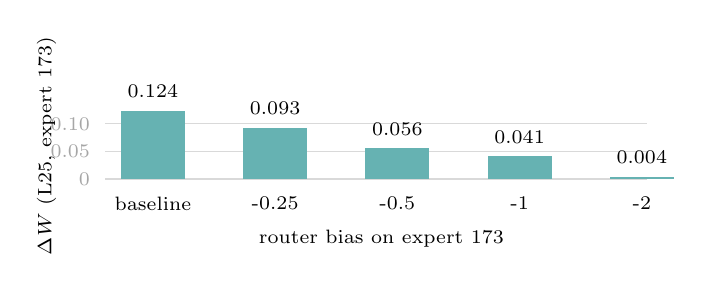
\begin{tikzpicture}[x=1.35cm,y=0.7cm]
\foreach \y in {0,0.05,0.10}{\draw[gray!30] (0,\y*10) -- (5.1,\y*10);
  \node[font=\scriptsize,gray!70,anchor=east] at (-0.05,\y*10){\y};}
\node[font=\scriptsize,rotate=90] at (-0.55,0.6){$\Delta W$ (L25, expert 173)};
\foreach \x/\v/\lab in {0/0.124/baseline,1/0.093/-0.25,2/0.056/-0.5,3/0.041/-1,4/0.004/-2}{
  \fill[teal!60] (\x*1.15+0.15,0) rectangle (\x*1.15+0.75,\v*10);
  \node[font=\scriptsize] at (\x*1.15+0.45,\v*10+0.35){\v};
  \node[font=\scriptsize,anchor=north] at (\x*1.15+0.45,-0.15){\lab};
}
\node[font=\scriptsize,anchor=north] at (2.6,-0.75){router bias on expert 173};
\end{tikzpicture}
\caption{Generation-block A$-$B routing difference for expert 173 at layer 25
as the router bias on index 173 (applied in all 40 routers) is swept from
baseline to $-2$. The expert's routing
collapses dose-dependently while the model's refusals persist at every
level.}
\label{fig:dose}
\end{figure}

\subsection{Aggregate top-ranked prefill experts are largely a padding artifact}
\label{sec:filler}

Read naively, the prefill block appears led by expert 173 at layer 1
($\Delta W=0.068$). The per-token decomposition shows this is mostly the
repeated filler piece: excluding it, the layer-1 figure falls to 0.0004, and
the other top aggregate prefill rows (expert 222 at layer 2, expert 36 at
layer 22) collapse similarly. The prompt-side candidates that survive the
correction are expert 218 at layer 14 ($0.025\to0.022$), expert 173 at layer
25 ($0.037\to0.046$), and expert 45 at layer 19 ($0.030\to0.034$). We
therefore rest the safety read on the generation block and record the
aggregate top-ranked prefill expert as a measurement caution: token-count padding can
fabricate a prefill expert that a per-token decomposition dissolves.

\section{Discussion}
\label{sec:discussion}

\paragraph{What the intervention establishes.}
Three results point the same way, and the suppression is the causal one. One
expert leads the routing separation, but it leads a set; the set tracks
consequence across topics; and biasing the leading expert's index to
near-zero routed mass, in every router, leaves the refusals in place while
routing reallocates to the rest of the set. A behavior owned by a single
expert should weaken when that expert is removed, and the removal here
contains that expert; this one persists unchanged. In this model, harm-refusal is a
property of a distributed set of experts that survives the loss of its most
active member. This is the expert-routing counterpart of the
distributed-representation expectation
\citep{elhage2022superposition,bricken2023monosemanticity} and stands against
a strict single-locus reading of refusal carried over from dense models
\citep{arditi2024refusal}. The contrast with \citet{lai2025safex} we take to
be setup-dependent: a single-expert intervention that fails to bypass refusal
here may succeed in another model, prompt regime, or with a multi-expert
intervention. What this run shows is that removing the strongest expert, with its
same-index experts, leaves refusal on this set intact.

\paragraph{Implication for safety auditing and intervention.}
The finding sets the granularity at which router-level safety work is
informative in this model. Monitoring the single most active
refusal-associated expert would report a large change under an intervention
that leaves refusal intact, and ablating it would leave refusal untested;
telemetry-based auditing \citep{lv2026routescan} and expert-level ablation
studies should therefore be read at the level of expert sets, and a
single-expert result, positive or negative, leaves open where refusal lives. The same logic bounds the attack surface: in this model
disabling the leading expert leaves refusal in place, and the routing that
reappears under suppression is the reason.

\paragraph{Scope of the causal claim.}
The suppression removes expert index 173 in all 40 routers and finds the
removed set dispensable. Because that set contains the leading expert, 173 at
layer 25, the leading expert is dispensable too, on the assumption that
removing fewer experts does not remove more of the behavior; a
layer-restricted suppression would test that assumption directly. The
intervention does not isolate the leading expert, and the same-index
assumption it rests on, that a shared index is a harmless way to name 40
unrelated experts at once, is one this paper's own Table~\ref{tab:gen-leaders}
declines to make when it ranks 173 at layer 25 and 173 at layer 13
separately. The joint necessity of the set (experts 45, 189, 157, 122 and
the others that absorb the load) remains untested, so the result covers
removal of the strongest expert's index. The behavioral read is a direct
reading of generated text on a small set; benchmarked refusal rates lie
outside the study. The result is a structural observation about where refusal-associated
routing lives in this model.

\section{Limitations}
\label{sec:limits}

Six and twelve prompts with one greedy trajectory each yield point estimates
with no sampled spread and no significance test, and per-prompt differences
can depend on tie-breaking; the ``still refuses'' verdict is the author's
reading of the generated text. One expert index was suppressed, in all 40 routers, so the leading expert
was never removed alone and the joint contribution of the set is untested. The control is bucketed, with intent matching in place of token pairing, so
its finance-versus-consequence separations are weaker evidence than the
matched pairs. The study covers one base model at one
quantization; whether refusal-reduced fine-tunes or other MoE families show
the same distributed pattern or a localizable expert \citep{lai2025safex} is
not addressed here.

\section{Conclusion}
\label{sec:conc}

In base \textsc{Qwen3.5-35B-A3B}, harm-refusal routes through a distributed
set of experts. One expert leads the redflag-minus-benign routing difference,
but biasing its index to near-zero routed mass in every router leaves the
refusals intact, because the surrounding consequence-and-duty set absorbs the
load. Refusal-associated
routing in this model is distributed, and the most active expert is
dispensable for refusal and an insufficient target for monitoring or attack.
Router-level safety analyses, whether they aim to audit, ablate, or attack,
should be read at the level of expert sets, and the unit an intervention
removes should be named as it was applied; a result about the single most
active expert speaks for that expert alone.

\section*{Data and Code Availability}
\addcontentsline{toc}{section}{Data and Code Availability}

The numbers in this paper are transcribed from the analysis tables of a
single capture session and are listed claim-by-claim, with source files, in
the accompanying \texttt{SOURCES.md}. The supporting data accompany the paper
in the \texttt{data/} directory: the run's results write-up and journal, the
all-layer A$-$B difference tables, the per-token decomposition that backs the
filler-artifact correction, the finance-versus-consequence bucket tables, the
expert-173 dose-response tables, the generated openings under suppression,
and the prompt sets. Raw router tensors (\texttt{.npy}) were not retained in
version control by project policy; the analysis tables above are derived from
them and substantiate the reported statistics. The routing reconstruction
satisfies $W=S\cdot Q$ per token set. No new model training was performed.

\section*{Ethical Considerations}

This work studies how a model refuses, using a small set of synthetic redflag
prompts (drug misuse, a prompt-injection attempt, and a financial
``sure-thing'') that the model refused at every intervention level. We
release the prompts and the model's refusals; no completion in this study
provides operational harm, and the suppression result is reported because it
fails to bypass refusal. The purpose is defensive: to establish whether
refusal in an MoE router is concentrated enough to be a single point of
failure for auditing or attack. The finding that it is distributed argues
against a single-expert attack surface in this model, and the claim is
limited to this model.

\section*{AI Collaboration Statement}
\addcontentsline{toc}{section}{AI Collaboration Statement}

Generative AI (Anthropic's Claude) was used as a tool in preparing this
manuscript: to assist with drafting and revising prose, organizing the
manuscript, and locating and formatting the bibliography. All experiments,
captures, and numerical results are the author's; every reported value was
traced to a source capture (see \texttt{SOURCES.md}), and every reference was
verified by the author against its authoritative record. No AI system is an
author. The author reviewed the entire text and takes full responsibility for
its content.

\section*{Funding and Competing Interests}
\addcontentsline{toc}{section}{Funding and Competing Interests}

This work received no external funding. The author declares no competing
interests. The model studied is a third-party open-weights release used as-is
for measurement; the author has no affiliation with its creators.

\bibliographystyle{plainnat}
\bibliography{refs}

\end{document}
